\title{Gitをボトムアップから理解する}

\begin{document}

\lstset{language={sh},showspaces=false,rulecolor=\color[cmyk]{0, 0.29,0.84,0}}

\begin{frame}
  \titlepage
\end{frame}

\section*{Outline}
\begin{frame}
  \tableofcontents
\end{frame}

\section{ライセンス}

\begin{frame}
  \frametitle{オリジナルとライセンス}
  \begin{itemize}
  \item ``Git from the bottom up'' (Original: John Wiegley)\\
    \url{http://newartisans.com/2008/04/git-from-the-bottom-up/}
  \item ``Gitをボトムアップから理解する'' (日本語訳: O-Show)\\
    \url{http://keijinsonyaban.blogspot.jp/2011/05/git.html}
  \item ライセンス: CC-BY-SA (3.0) \\
    \url{http://creativecommons.org/licenses/by-sa/3.0/us/}
  \end{itemize}
\end{frame}

\section{導入: gitの世界}

\begin{frame}
  \frametitle{用語集}
  リポジトリ関連
  \begin{description}
  \item[リポジトリ] コミットの集合, ワーキングツリーのアーカイブ
  \item[インデックス] 変更を登録する場所, ステージングエリア, \alert{git独自}
  \item[ワーキングツリー] リポジトリのあるディレクトリ
  \end{description}
  コミット関連
  \begin{description}
  \item[コミット] ある時点でのワーキングツリーのスナップショット
  \item[ブランチ] \alert{コミット(群)の別名}, リファレンス
  \item[タグ] \alert{コミットの別名}, 常に同じコミットを指す
  \item[master] デフォルトのことが多い\alert{単なるブランチ}
  \item[HEAD] チェックアウトされているもの
    \begin{itemize}
    \item ブランチなら、コミット操作でブランチがアップデート
    \item 特定のコミットなら、(detached HEAD), タグ名でチェックアウトしたとき等
    \end{itemize}
  \end{description}
\end{frame}

\begin{frame}
  \frametitle{基本的な概念}
  \begin{center}
    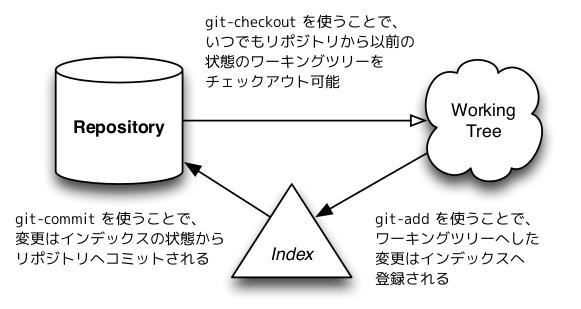
\includegraphics[height=.6\textheight]{4_ja.png}
  \end{center}
\end{frame}

\section{リポジトリ}

\begin{frame}
  \frametitle{gitでの作業}
  \begin{itemize}
  \item 作業はワーキングツリーで
  \item 1段落したら、変更をインデックスへ
  \item 変更がまとまったらコミット
  \end{itemize}
\end{frame}

\begin{frame}
  \frametitle{gitの基礎}
  \begin{alertblock}{}
    ディレクトリのスナップショットを保全する
  \end{alertblock}
\end{frame}

\begin{frame}
  \frametitle{blob: gitの基本オブジェクト}
  \begin{description}
  \item[中身] ファイルコンテンツ
  \item[名前] サイズと内容のSHA-1ハッシュ
  \end{description}
  \begin{alertblock}{}
    メタデータを一切保存しない
  \end{alertblock}
\end{frame}

\begin{frame}[fragile]
  \frametitle{blobの紹介}
\begin{lstlisting}
$ mkdir sample; cd sample
$ echo 'Hello, world!' > greeting 
$ git hash-object greeting
af5626b4a114abcb82d63db7c8082c3c4756e51b
$ git init
$ git add greeting
$ git commit -m ``Added my greeting''
$ git cat-file -t af5626b
blob
$ git cat-file blob af5626b
Hello, world!
\end{lstlisting}
\end{frame}

\begin{frame}
  \frametitle{tree: blobを保管}
  \begin{block}{}
    blobはtreeのleaf-nodeである
  \end{block}
\end{frame}

\begin{frame}[fragile]
  \frametitle{treeの表示(1)}
  \begin{lstlisting}
$ git ls-tree HEAD
100644 blob af5626b4a114abcb82d63db7c8082c3c4756e51b greeting
$ git rev-parse HEAD
588483b99a46342501d99e3f10630cfc1219ea32 # これはあなたのシステム上では別物になる
$ git cat-file -t HEAD
commit
$ git cat-file commit HEAD
tree 0563f77d884e4f79ce95117e2d686d7d6e282887
author John Wiegley <johnw@newartisans.com> 1209512110 -0400
committer John Wiegley <johnw@newartisans.com> 1209512110 -0400

Added my greeting 
\end{lstlisting}
\end{frame}

\begin{frame}[fragile]
  \frametitle{treeの表示(2)}
\begin{lstlisting}
$ git ls-tree 0563f77
100644 blob af5626b4a114abcb82d63db7c8082c3c4756e51b greeting
$ find .git/objects -type f | sort
.git/objects/05/63f77d884e4f79ce95117e2d686d7d6e282887
.git/objects/58/8483b99a46342501d99e3f10630cfc1219ea32
.git/objects/af/5626b4a114abcb82d63db7c8082c3c4756e51b 
$ git cat-file -t 588483b99a46342501d99e3f10630cfc1219ea32
commit
$ git cat-file -t 0563f77d884e4f79ce95117e2d686d7d6e282887
tree
$ git cat-file -t af5626b4a114abcb82d63db7c8082c3c4756e51b
blob
\end{lstlisting}
\end{frame}

\begin{frame}[fragile]
  \frametitle{手作業でtreeを作る}
  \begin{lstlisting}
$ rm -fr greeting .git
$ echo 'Hello, world!' > greeting
$ git init
$ git add greeting
$ git log # これは失敗する。まだコミットは存在しない!
fatal: bad default revision 'HEAD'
$ git ls-files --stage # index によって参照される blob を一覧表示する
100644 af5626b4a114abcb82d63db7c8082c3c4756e51b 0 greeting
  \end{lstlisting}
  \begin{block}{}
    同じファイルは同じblobになる
  \end{block}
\end{frame}

\begin{frame}[fragile]
  \frametitle{手作業でcommitを作る}
  \begin{lstlisting}
$ git write-tree # 一つの tree として index の内容を記録する
0563f77d884e4f79ce95117e2d686d7d6e282887
$ echo ``Initial commit'' | git commit-tree 0563f77
5f1bc85745dcccce6121494fdd37658cb4ad441f
$ echo 5f1bc85745dcccce6121494fdd37658cb4ad441f > .git/refs/heads/master
$ git update-ref refs/heads/master 5f1bc857
$ git symbolic-ref HEAD refs/heads/master
$ git log
commit 5f1bc85745dcccce6121494fdd37658cb4ad441f
Author: John Wiegley <johnw@newartisans.com>
Date: Mon Apr 14 11:14:58 2008 -0400

Initial commit 
  \end{lstlisting}
\end{frame}

\begin{frame}
  \frametitle{gitの全体構造}
  \begin{center}
    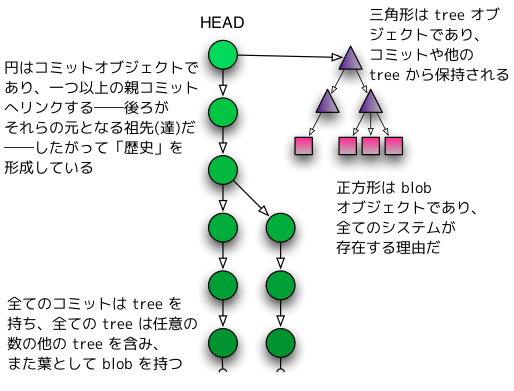
\includegraphics[height=.6\textheight]{12_ja.png}
  \end{center}
\end{frame}

\begin{frame}
  \frametitle{インデックス}
  \begin{center}
    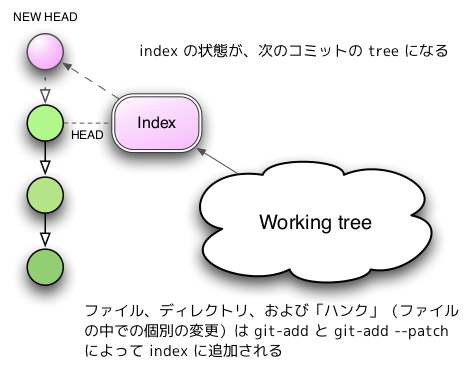
\includegraphics[height=.6\textheight]{20_ja.png}
  \end{center}
\end{frame}

\end{document}
